\section{Evaluation} \label{sec:evaluation}
Der zuvor dargestellte MoDiGen Ansatz, in dem Knoten und Kanten gleichwertig und einzeln im JSON-Format gespeichert werden, wird in Abbildung \ref{fig:Num-Char-Family-Tree-Model} Ecore gegenübergestellt. Dabei wird die Anzahl der Buchstaben, die gespeichert werden müssen, betrachtet und der Unterschied zwischen beiden Metamodellen Prozentual dargestellt. Die größte Reduzierung in der Anzahl der Zeichen findet beim Entfernen der Leerzeichen statt. Hier werden beim Speichern 58\% weniger Zeichen benötigt wenn das MoDiGen-Modell verwendet wird. Werden die Leerzeichen nicht entfernt sondern nur die Standardwerte benötigen MoDiGen und Ecore fast gleich viele Zeichen bei der Speicherung des gleichen Modells. Hier benötigt MoDiGen lediglich 2\% weniger Zeichen. Da bei Ecore aber standardmäßig die Leerzeichen und Standardwerte entfernt werden ist der letzte Vergleich am praxisnächsten. Hier benötigt MoDiGen 36\% weniger Zeichen als sein Konkurrent.
\begin{figure}[H]
\centering
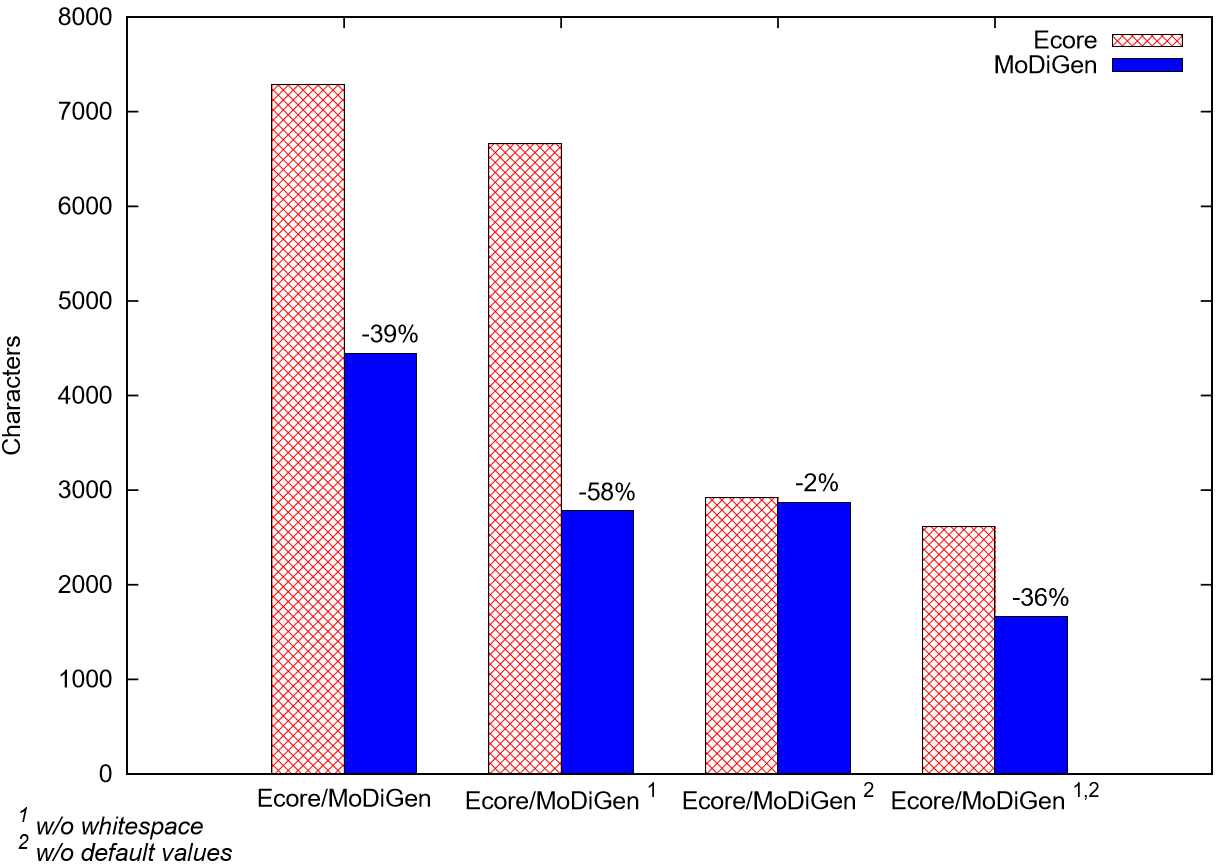
\includegraphics[width=\linewidth]{Abschnitte/Abbildungen/Grafiken/Num-Char-Family-Tree-Model}
\caption{Buchstabenanzahlvergleich aus dem Family Tree Beispiel}
\label{fig:Num-Char-Family-Tree-Model}
\end{figure}
Die Anzahl der zu speichernden Zeichen steht im Verhältnis zur Anzahl der im Modell verwendeten Knoten. 
In der Abbildung \ref{fig:Characters-and-Nodes} wird dieses Verhältnis grafisch dargestellt. In der Darstellung lässt sich erkennen, dass in Modellen in denen wenig Knoten benötigt werden kein großer Unterschied zwischen Ecore und MoDiGen liegt. Steigt die Anzahl der Knoten aber wird der Unterschied zwischen den beiden Modellen immer größer. Diese Auswertung liegt einem Praxisbeispiel zu Grunde in dem Knoten verwendet wurden, die jeweils miteinander verbunden sind. Wie zuvor festgestellt lässt sich eine starke Reduktion der Zeichen erreichen indem die Standardwerte und die Leerzeichen entfernt werden. Daher wurden diese beiden Reduktionen in diesem Beispiel angewandt.\\
Der Unterschied in der Zeichenanzahl liegt der Art der Speicherung der Kanten zu Grunde, daher relativiert sich dieser Unterschied, wenn nur wenig Kanten benötigt werden. In einer Erweiterung des Praxisbeispiels wurden 10.000 Knoten betrachtet die jeweils miteinander verbunden sind. Für dieses Beispiel wurde der Speicherbedarf ermittelt. Hier benötigte Ecore 5,58 Gigabyte und MoDiGen 3,6 Megabyte.\\
Ein weiteren Vorteil hat MoDiGen durch die Verwendung des JSON-Formats. Dank der horizontalen Skalierungsmöglichkeiten die mit Datenbanken wie CouchDB, MongoDB oder RavenDB genutzt werden kann, können sehr große Modelle auch aufgeteilt werden. \textit{Horizontale Skalierung bedeutet...} Eine Teilung wäre bei der Verwendung des XML-Formats nicht möglich. 


\begin{figure}[H]
\centering
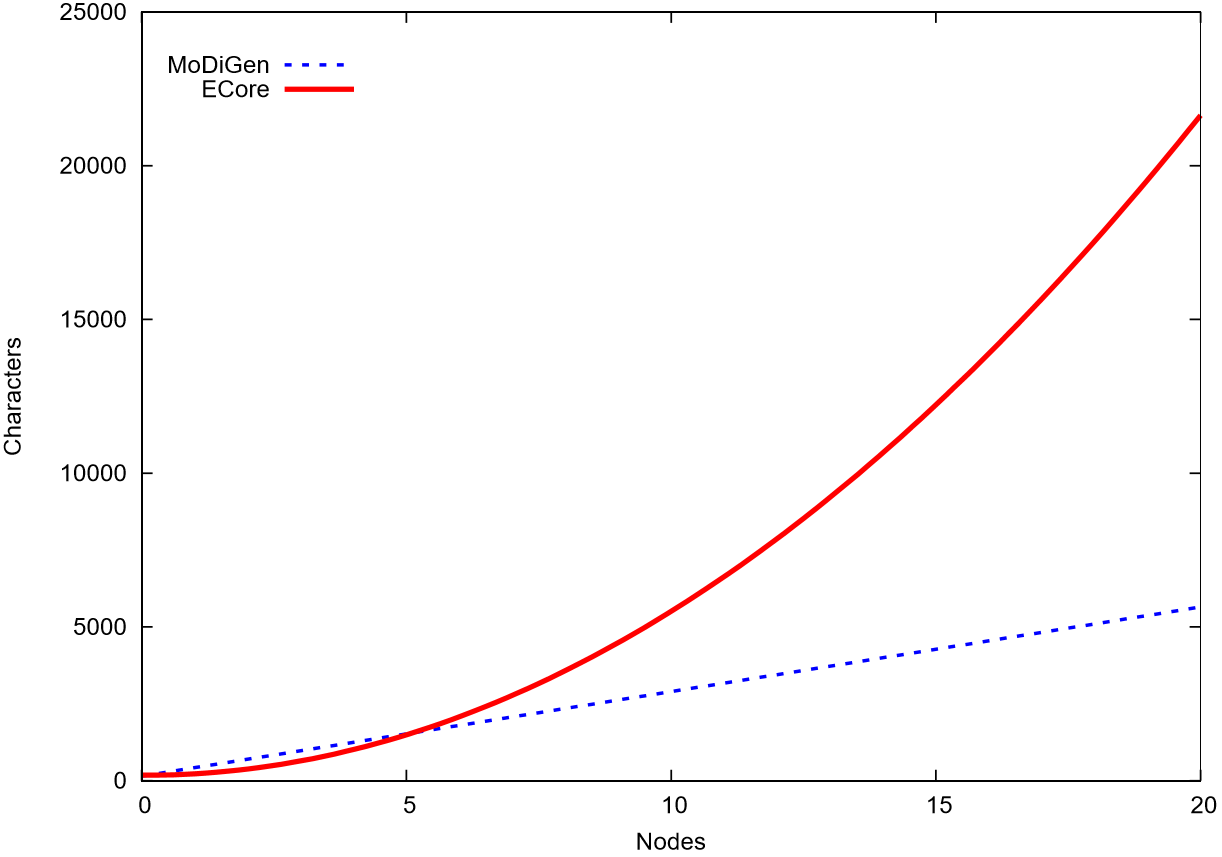
\includegraphics[width=\linewidth]{Abschnitte/Abbildungen/Grafiken/Characters-and-Nodes}
\caption{Buchstabenmenge im Verhältnis zu erzeugten Knotenpunkte}
\end{figure}
